\renewcommand{\thefigure}{\Asbuk{section}.\arabic{figure}}
\renewcommand{\thetable}{\Asbuk{section}.\arabic{table}}
\renewcommand{\thelstlisting}{\Asbuk{section}.\arabic{lstlisting}}

\addcontentsline{toc}{section}{Приложение А (обязательное) 
  Базовая модель и результаты её имитации}
\section*{ПРИЛОЖЕНИЕ A \\ 
  (обязательное) \\ 
  Базовая модель и результаты её имитации}
\label{sec:appendix_a}

\pagestyle{fancy}
\fancyhf{}  % clear all header and footer fields
\fancyfoot[R]{\thepage}
\renewcommand{\headrulewidth}{0pt}
\renewcommand{\footrulewidth}{0pt}

\setlength{\headheight}{10mm}
\setlength{\headsep}{\baselineskip}
\chead{Продолжение приложения \Asbuk{section}}

\thispagestyle{plain}

\setcounter{section}{1}
\setcounter{figure}{0}
\setcounter{table}{0}
\setcounter{lstlisting}{0}

\lstinputlisting[caption=Исходный текст базовой GPSS-модели,
basicstyle=\small\ttfamily,
label=lst:base_model]{code/base.txt}

\begin{figure}[h!]
  \centering
  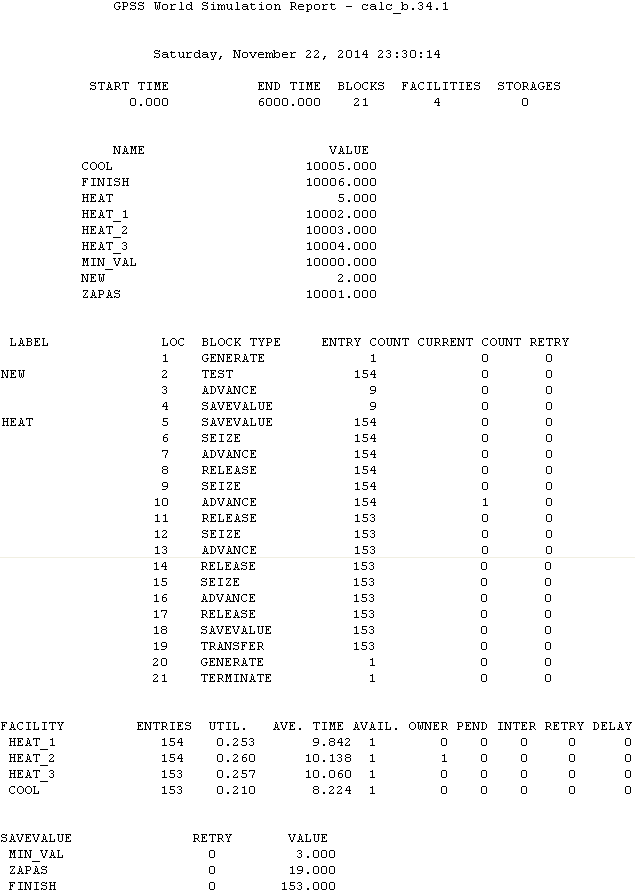
\includegraphics[width=150mm]{pic/base_report}
  \caption{Статистика базовой GPSS-модели}
  \label{pic:base_report}
\end{figure}
